\subsection{Генерация текста}

\subsubsection{Введение}
Широко известно, что изучение и использование языка требует наличия контекста, для того чтобы быть эффективным средством коммуникации между участниками диалога. Особенно необходим контекст при изучении студентами новых слов иностранного языка, одного перевода зачастую недостаточно для обеспечения полного понимания семантики слова или фразы. По этой причине при изучении нового материала необходимо обеспечить учащихся примерами использования, продемонстрировать контекст применения и смысловую окраску слова.

Подбор фрагментов текста с использованием конкретного слова вручную является трудоемкой и неэффективной задачей. При изучении 3 слов в день за один год потребовалось бы найти свыше 16,000 предложений с примерами использования, чтобы наполнить мобильное приложение данными (из расчета 3 слова в день $\times$ 5 примеров на слово $\times$ 365 дней $\times$ 3 уровня сложности).

Одним из решений было бы производить поиск слов в различных электронных ресурсах или книгах, извлекать предложение, которое содержит слово и таким образом автоматизировать процесс создания базы примеров. Однако такой подход имеет ряд недостатков: большинство текстов хорошего качества защищены авторскими правами, набор источников все равно нужно подбирать вручную, а тематика собранных предложений может быть неуместна для использования в обучающем приложении.

Мы подходим к решению этой проблемы с помощью нейронных сетей и алгоритмов машинного обучения. Классическим методом генерации текста является использование рекуррентных нейронных сетей. Относительно недавно были представлены способы использования генеративно-состязательных сетей для решения этой задачи, превосходящие предыдущие подходы по качеству результирующего текста. В последующих пунктах мы детальнее рассмотрим технологии генерации текста и их применение в создании набора примеров для использования в мобильном приложении.

\subsubsection{Генерация текста с использованием RNN}
Рекуррентные нейронные сети являются мощным инструментом для моделирования последовательностей данных, как было рассмотрено в предыдущих пунктах. RNN сети запоминают и используют информацию, обработанную в прошлом, что позволяет им лучше ориентироваться в контексте. Однако на протяжении долгого времени они практически не использовались в области генерации текста из--за сложностей, возникающих при обучении. Проблемы возникают из-за крайне нестабильным отношением между параметрами и изменениями внутреннего состояния и проблемы угасающих/увеличивающихся градиентов\cite{bengio1994learning}. Тем не менее, эту проблему удалось преодолеть используя другой подход к оптимизации: вместо обычного градиентного спуска, который задействует первые производные, использовать модифицированный метод Ньютона с производными второго порядка\cite{martens2010deep}.

Стандартная рекуррентная нейронная сеть может быть формализована следующим образом. На вход подается последовательно векторов $\mathbf{x} = (\mathbf{x}_1, \dots, \mathbf{x}_T)$, по этим векторам RNN вычисляет последовательность внутренних состояний $\mathbf{h} = (\mathbf{h}_1, \dots, \mathbf{h}_T)$ и последовательность выводов $\mathbf{o} = (\mathbf{o}_1, \dots, \mathbf{o}_T)$. Последовательности $\mathbf{h}$ и $\mathbf{o}$ вычисляются из уравнений
$$\mathbf{h}_t = \tanh(W_{hx}x_t + W_{hh}h_{t - 1} + b_h),$$
$$\mathbf{o}_t = W_{oh}h_t + b_o.$$

Здесь матрица весов $W_{hx}$ отвечает за трансформацию входных данных во внутреннее состояние, матрица $W_{hh}$ необходима для обновления внутреннего состояния в соответствии с предыдущим, $W_{oh}$ --- для преобразования внутреннего состояния в выходную последовательность. Векторы $\mathbf{b}_h$ и $\mathbf{b}_h$ отвечают за bias.

Для улучшения результатов работы при генерации текста в стандартную модель, представленную выше, вносится ряд изменений.

Матрица $W_{hh}$ замещается на тензор $W_{hh}^{(x_t)}$, чтобы для каждого символа можно было определить свою матрицу весов. Если размерность входного вектора $\mathbf{x}_t$ равна $M$, то $W_{hh}^{(x_t)}$ можно определить так:
$$W_{hh}^{(x_t)} = \sum_{m = 1}^{M} x_t^{(m)}W_{tt}^{(m)}.$$

На практике же хранение тензоров таких размерностей может быть недопустимым. Поэтому матрица $W_{hh}^{(x_t)}$ разделяется на 3 части:
$$W_{hh}^{(x_t)} = W_{hf} \cdot \operatorname{diag}(W_{fx}x_t) \cdot W_{fh}.$$
А сама модель меняется следующим образом:
$$f_t = \operatorname{diag}(W_{fx}x_t) \cdot W_{fh} h_{t - 1},$$
$$h_t = \tanh(W_{hf}f_t + W_{hx}x_t).$$

Такая модифицированная рекуррентная нейронная сеть называется мультипликативной RNN (MRNN)\cite{sutskever2011generating}.

Определенная таким образом модель может использоваться для генерации последовательности символов. По входной последовательности $\mathbf{x}$ RNN дает последовательность условных вероятностей $P(\mathbf{x}_{t + 1}|\mathbf{x}_0, \dots, \mathbf{x}_t) = \operatorname{Softmax}(\mathbf{o}_t)$. Цель обучения --- максимизация общей вероятности на обучающей выборке:
$$\sum_{t = 0}^{T - 1} \log P(x_{t + 1}| x_0, \dots, x_t).$$

В результате MRNN позволяет генерировать текст довольно высокого качества даже при небольшом количестве узлов и размере обучающей выборки.

\subsubsection{Применение LSTM сетей для генерации текста}
Как уже упоминалось в предыдущем пункте, обучение RNN сетей на длинных последовательностях связано с проблемой затухающих/увеличивающихся градиентов. В предыдущем пункте мы рассмотрели решение этой проблемы с помощью применения модифицированного метода Ньютона второго порядка вместо обычного градиентного спуска. В этом пункте мы рассмотрим более прогрессивное решение в виде использования LSTM блоков, устройства которых мы касались в пункте \ref{section:rnn-in-asr}.

Модель представляет собой RNN сеть, которая по входному символу в момент времени $t$ и текущему внутреннему состоянию $\mathbf{h}_t$ дает вероятностное распределение для следующего символа. Сеть состоит из модифицированных LSTM узлов, устройство которых мы рассмотрим далее. Таким образом сеть позволяет генерировать текст посимвольно до тех пор, пока не будет сгенерирован конец последовательности, либо сработает нужное нам условие.

Рассмотрим структуру модифицированного LSTM узла, которая была представлена в \cite{wen2015semantically} и изображена на рисунке \ref{fig:semantic-controlled-lstm}.
\begin{figure}[h]
	\centering
	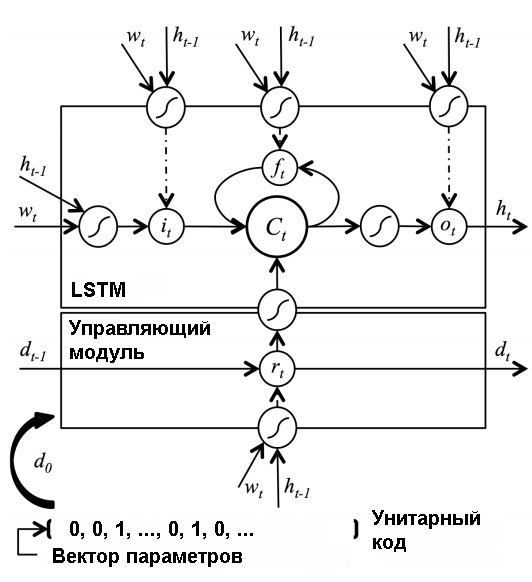
\includegraphics[width=0.4\textwidth]{semantic-controlled-lstm}
	\caption{Структура модифицированного LSTM узла.}
	\label{fig:semantic-controlled-lstm}
\end{figure}

Ключевая особенность архитектуры LSTM заключается в возможности управлять памятью узлов при помощи специальных входов, отвечающих за сохранение, удаление и модификацию хранящейся в памяти информации. Дополнительный модуль управления, изображенный снизу, позволяет управлять значением фразы на выходе. Желаемое значение текста кодируется унитарным кодом\footnote{Унитарный код --- способ кодирования, при котором группа битов содержит лишь одну единицу, а остальные ячейки заполнены нулями. Например, число 3 при таком кодировании представляется в виде \ldots001000.} и подается в виде управляющего вектора $\mathbf{d}$. Этот дополнительный модуль управляет содержанием предложения для достижения соответствия результата входным параметрам. На каждом этапе определяется, какая информация должна быть сохранена для будущих шагов, а все остальные нерелевантные данные отбрасываются.

Такая архитектура легко расширяется на случай глубоких нейронных сетей путем увеличения количества LSTM узлов.

Для дальнейшего улучшения качества результатов вводится еще одна модификация. В базовом варианте архитектуры при генерации новых символов сеть руководствуется только данными из прошлого. Однако нередко смысловая нагрузка в предложении распределена неравномерно, и бывает полезным знать то, что будет стоять за текущим словом. Двунаправленные LSTM сети\cite{graves2013hybrid} в теории могли бы решить эту проблему, однако их внедрение в представленную выше архитектуру весьма нетривиально, поскольку процесс генерации выходных символов происходит последовательно. Поэтому вместо внедрения BLSTM сетей происходит обучение ещё одной идентичной сети на данных, представленных в обратном порядке. С помощью этого приема становиться возможным оценивать выходную последовательность не только по данным, предшествующим текущему элементу последовательности, но и учитывать следующие элементы.

Архитектура такой системы способна генерировать реалистичные фрагменты текстов в соответствии с заданным желаемым вектором смысловых характеристик. Модель демонстрирует превосходство в качестве сгенерированных предложений над предыдущими подходами\cite{wen2015semantically}.

\subsubsection{Генерация текста при помощи GAN сетей}
Генеративно-состязательные сети (generative adversarial networks, GAN) --- архитектура нейронных сетей для генерирования данных с использованием средств глубокого обучения, таких, как, например, сверточные нейронные сети. Генерирование нового контента -- это задача обучения без учителя, которая включает в себя обнаружение и запоминание закономерностей или шаблонов во входных данных таким образом, чтобы впоследствии модель могла генерировать новые объекты. Сгенерированные данные должны быть максимально правдоподобны, чтобы нельзя было определить, были ли они созданы при помощи нашей модели или же происходят из входного набора данных.

В сущности, генеративно-состязательные сети --- это разумный способ свести задачу создания генеративной модели к задаче обучения с учителем, состоящей из двух подмоделей: генеративной модели, которая обучается созданию новых данных и дискриминативной модели, которая старается отличить «подлинные» образцы от сгенерированных. Две модели обучаются параллельно, постоянно пытаясь обыграть друг друга. Процесс обучения завершается тогда, когда дискриминативная модель ошибается приблизительно в половине случаев, что означает, что создаются достаточно правдоподобные образцы.

Впервые генеративно-состязательные сети были представлены в 2014 году Ian Goodfellow и коллегами\cite{gan-introduction}, а некоторые дополнения, такие, как StyleGAN были разработаны совсем недавно -- в 2018 году\cite{gan-stylegan}. Этот вид сетей активно развивается, постоянно меняется и имеет уникальные возможности, в числе которых: создание фотореалистичных изображений заданных объектов (например, человеческих лиц), синтез голоса, поднятие разрешения фотографий\cite{gan-upscaling} или трансформацию одних изображений в другие.

Общая структура генеративно--состязательных сетей представлена на рисунке \ref{label}.
\begin{figure}[h]
	\centering
	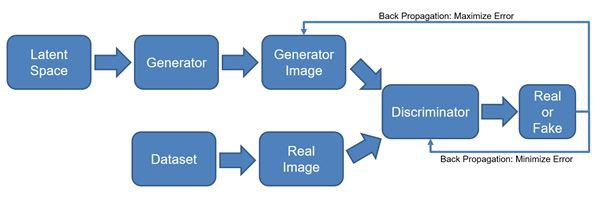
\includegraphics[width=0.7\textwidth]{gan-architecture}
	\caption{Архитектура GAN сети.}
	\label{fig:gan-architecture}
\end{figure}

В процессе обучения генеративная часть сети пытается минимизировать функцию (\ref{eq:gan-loss}), в то время как дискриминативная часть пытается её максимизировать. 
\begin{equation}
\label{eq:gan-loss}
\mathcal{L}_{GAN} = E_x[log(D(x))] + E_z[log(1 - D(G(z)))]
\end{equation}

Здесь:
\begin{itemize}
	\item $D(\cdot)$ -- вероятность того, что изображение является подлинным;
	\item $E$ -- мат. ожидание;
	\item $G(\cdot)$ -- вывод генератора;
	\item $x$ -- экземпляр из выборки подлинных данных;
	\item $z$ -- случайный шум.
\end{itemize}

Сложность использования GAN сетей для генерации текста связана с тем, что данный класс сетей изначально направлен на работу с визуальными данными, а текст имеет дискретную природу. Тем не менее, результаты исследований\cite{zhang2017adversarial} демонстрируют высокую перспективность этого подхода.

В качестве сети--генератора используется LSTM сеть, а в качестве дискриминатора --- сверточная сеть. Архитектура CNN--сеть дискриминатора позаимствована из работы \cite{zhang2015sensitivity} и представлена на рисунке \ref{fig:cnn-discriminator}.

\begin{figure}[h]
	\centering
	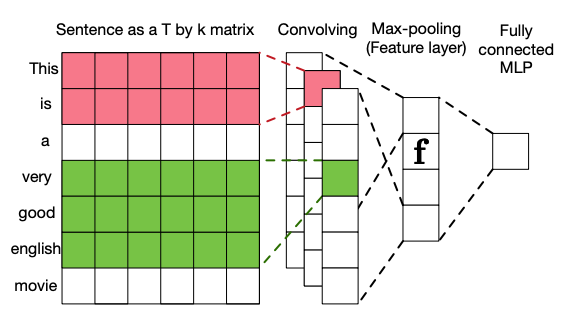
\includegraphics[width=0.7\textwidth]{cnn-discriminator}
	\caption{Архитектура CNN сети дискриминатора.}
	\label{fig:cnn-discriminator}
\end{figure}

Сначала предложение преобразуется в матрицу путем конкатенации векторного представления каждого слова, после чего проходит через серию фильтров. Векторное представление может быть получено с помощью модели word2vec\cite{mikolov2013distributed} или GloVe\cite{pennington2014glove}. Каждый фильтр направлен на извлечение конкретного лингвистического признака. Слой max-pooling необходим для отбора наиболее важных признаков. В конце сети находятся полносвязные слои.

Рекуррентная сеть--генератор, использующая LSTM, переводит входной вектор признаков $\mathbf{z}$ в синтезированное предложение $s$. Так же как и предыдущих пунктах, генерация предложения происходит посимвольно, вероятность получения предложения $s$ для заданного вектора $\mathbf{z}$ может быть выражена формулой
$$P(s | \mathbf{z}) = P(w_1 | \mathbf{z}) \prod_{t=2}^{T} P(w_t | w_1, \dots, w_{t - 1}, \mathbf{z}).$$
Здесь $w_t$ означает символ, полученный на $t$-том шаге. Первый символ определяется по входному вектору $\mathbf{z}$ детерминированно.

Такая архитектура показывает\cite{zhang2017adversarial} значительное улучшение в результатах генерации текста в сравнении с предыдущими подходами. Архитектура GAN сети позволяет создавать предложения, обладающие высокой реалистичностью, а модель может адаптироваться и обучаться, запоминая наиболее правдоподобные текстовые фрагменты.

\subsubsection{Вывод по главе}
В данной главе был проведен сравнительный анализ ведущих алгоритмов в области генерирования текста. Задача автоматической генерации текста возникает в сфере изучения иностранных языков в связи с необходимостью предоставить большую базу примеров, по которой обучающиеся смогут лучше разобраться в контексте использования слов и смысловой составляющей. Синтез текста при помощи нейронных сетей получил наибольшее развитие лишь в относительно недавний период времени. Мы рассмотрели использование RNN и LSTM сетей, а также новый экспериментальный подход в виде генеративно--состязательных сетей. У каждого подхода есть свои преимущества. Так, архитектура с использованием LSTM сетей позволяет генерировать тексты, органично включающие в себя заданную информацию и смысл. GAN--сети же, хоть и обладают на данный момент более ограниченными возможностями, способны порождать более реалистичные предложения. Практическое применение технологии генерация текста с заданными параметрами будет рассмотрено в следующих разделах.
